%----------------------------------------------------------------------------------------
%	PACKAGES AND OTHER DOCUMENT CONFIGURATIONS
%----------------------------------------------------------------------------------------

\documentclass[9pt]{developercv} % Default font size, values from 8-12pt are recommended
\usepackage{graphicx}
\usepackage[export]{adjustbox}
%----------------------------------------------------------------------------------------

\begin{document}

%----------------------------------------------------------------------------------------
%	TITLE AND CONTACT INFORMATION
%----------------------------------------------------------------------------------------

\begin{minipage}[t]{0.3\textwidth} % 45% of the page width for name
	\vspace{-\baselineskip} % Required for vertically aligning minipages
	\colorbox{black}{{\Huge\textcolor{white}{\textbf{\MakeUppercase{Ionut Daniel}}}}}
	
	\colorbox{black}{{\Huge\textcolor{white}{\textbf{\MakeUppercase{Fagadau}}}}}
	
	\vspace{6pt}
	
	{\Large 17 Gennaio 1999 \\ Dorohoi, Romania} % Career or current job title
\end{minipage}
\begin{minipage}[t]{0.22\textwidth} % 27.5% of the page width for the first row of icons
	\vspace{-\baselineskip} % Required for vertically aligning minipages
	
	% The first parameter is the FontAwesome icon name, the second is the box size and the third is the text
	% Other icons can be found by referring to fontawesome.pdf (supplied with the template) and using the word after \fa in the command for the icon you want
	\icon{MapMarker}{12}{Trecate, Novara}\\
	
	\icon{Github}{12}{\href{https://github.com/Mooyeee}{Daniel Fagadau}}\\
	
	\icon{Phone}{12}{+39 3890989121}\\
\end{minipage}
\begin{minipage}[t]{0.3\textwidth}
\vspace{-\baselineskip}
\icon{At}{12}{danielfagadau@gmail.com}\\

	\icon{Linkedin}{12}{\href{https://www.linkedin.com/in/daniel-fagadau/}{daniel-fagadau}} \\	
\end{minipage}
\begin{minipage}[t]{0.2\textwidth}
\vspace{-\baselineskip}
\noindent
\centering
\vspace{-20mm}{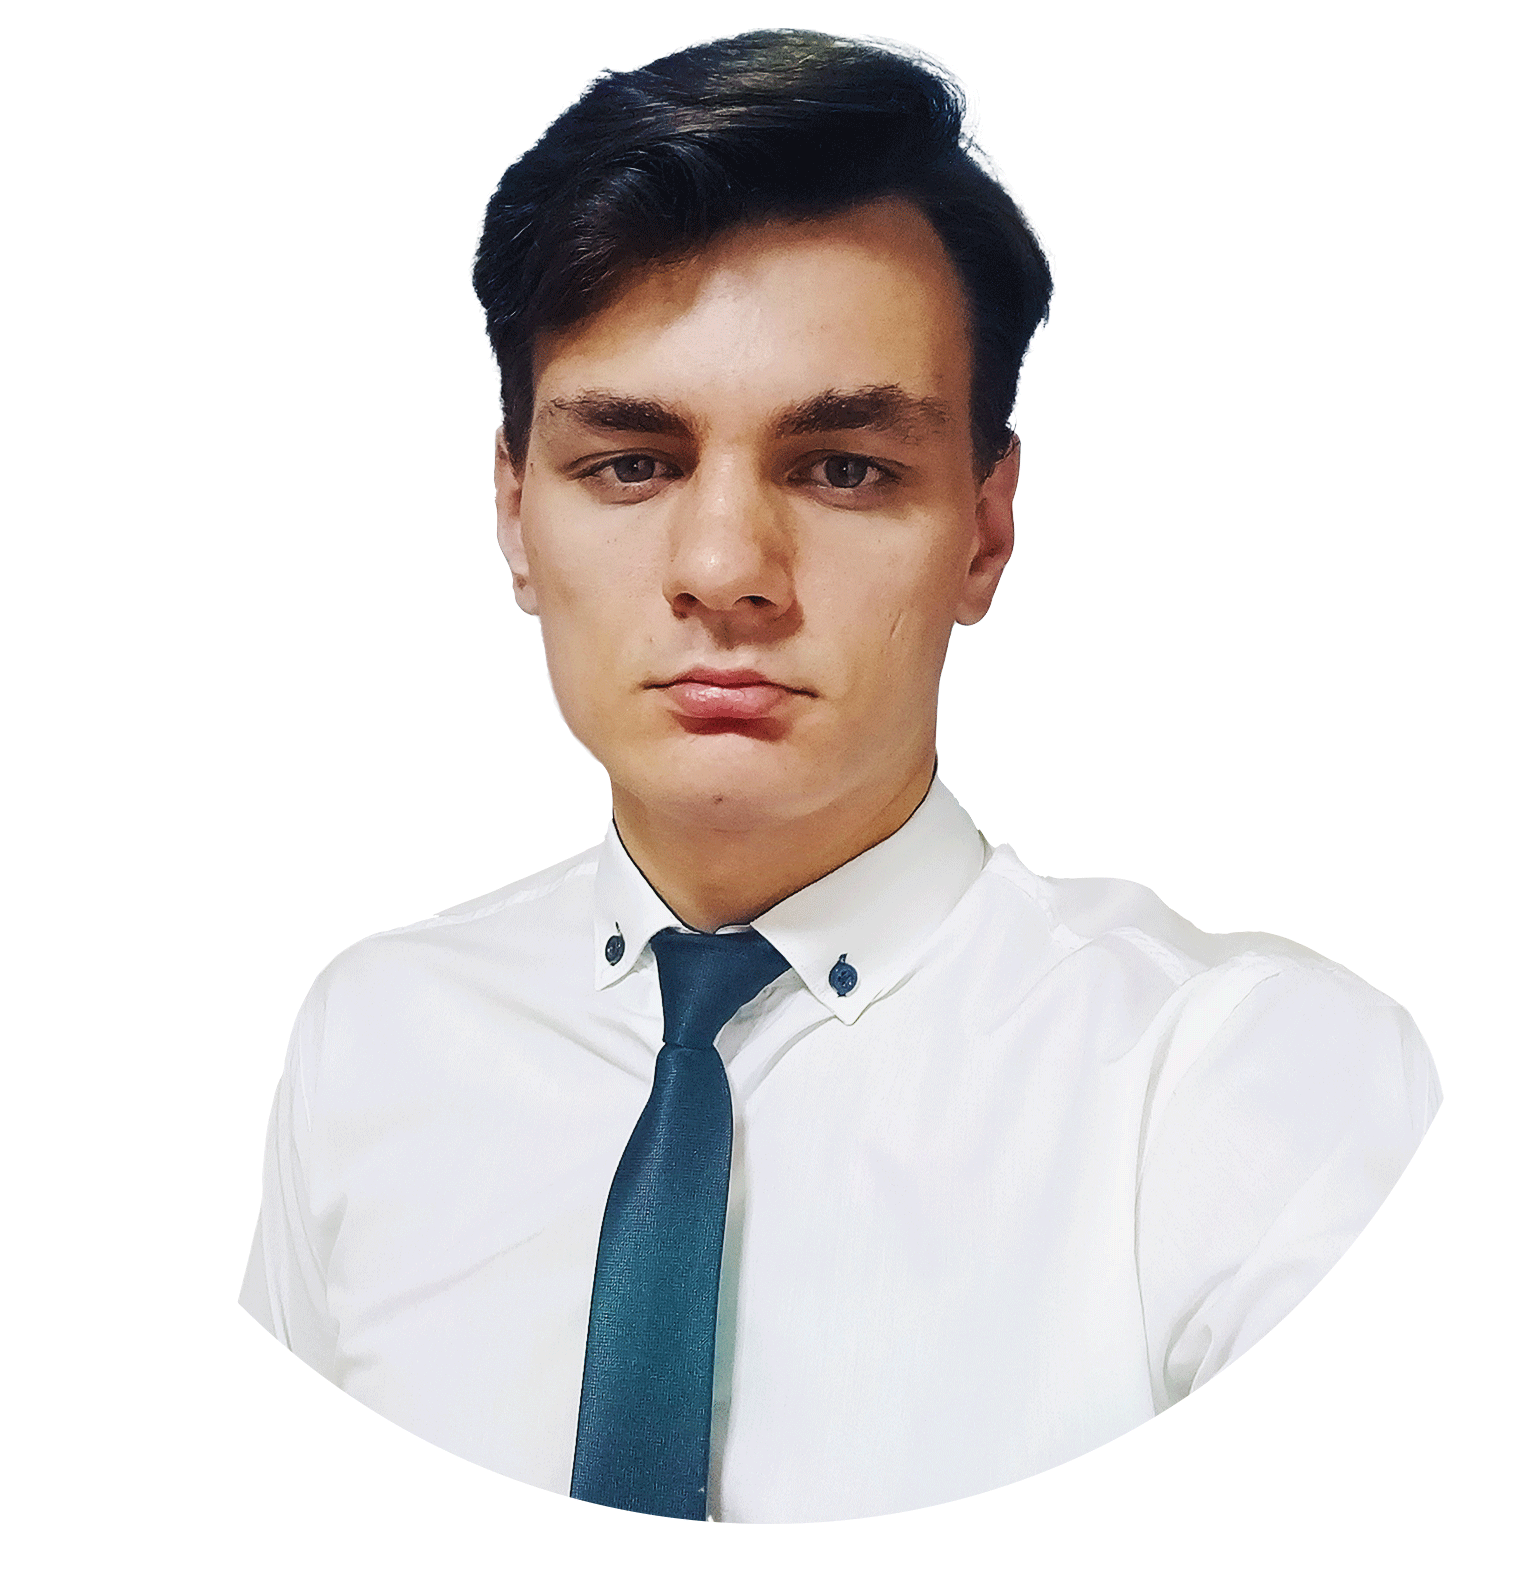
\includegraphics[scale=0.045, center]{foto_cv}}
\end{minipage}

\vspace{0.5cm}


%----------------------------------------------------------------------------------------
%	EXPERIENCE
%----------------------------------------------------------------------------------------

\cvsect{Esperienza professionale}

\begin{entrylist}

\entry
	{3/4/2023 \\ 3/6/2023 \\\footnotesize{smart working}\\\footnotesize{full remote}}
	{Borsa Ricerca: Reingegnerizzazione/Testing MindBlooming}
	{Università degli Studi di Milano - Bicocca}
	{A seguito di uno studio di usabilità svolto dal dipartimento di Teoria e Tecnologia della Comunicazione UniMiB, è stato svolto un refactoring generale della codebase dell’app MindBlooming con conseguente reingegnerizzazione, testing e miglioramento generale dell’interfaccia grafica e dell’esperienza utente.\\ \texttt{Flutter}\slashsep\texttt{Dart}\slashsep\texttt{Java}}

\entry
	{22/3/2023 \\ 19/5/2023}
	{Docente Algoritmi e Programmazione [E3501Q067]}
	{Università degli Studi di Milano - Bicocca}
	{Ho svolto le lezioni in laboratorio del corso di Algoritmi e Programmazione del secondo anno del corso di Laurea Triennale in Matematica. Le lezioni prevedevano il chiarimento di eventuali dubbi degli studenti sugli argomenti trattati nelle lezioni frontali quali classi e istanze in Java, associazioni tra classi, incapsulamento, overloading e costruttori, ereditarietà, classi astratte, interfacce e polimorfismo. Sono stati usati sia editor di testo semplici che l’IDE Eclipse.\\ \texttt{Java}\slashsep\texttt{Eclipse}}

\entry
	{20/3/2023 \\ 23/5/2023}
	{Docente Lab. di Matematica e Informatica [E3501Q066]}
	{Università degli Studi di Milano - Bicocca}
	{Ho svolto le lezioni in laboratorio del corso di Laboratorio di Matematica e Informatica del primo anno del corso di Laurea Triennale in Matematica. Le lezioni prevedevano il chiarimento di eventuali dubbi degli studenti sugli argomenti trattati nelle lezioni frontali riguardanti i primi approcci alla programmazione con Java e quindi i concetti di programma, linguaggi, tipi, variabili, operatori, controllo del flusso e metodi.\\ \texttt{Java}\slashsep\texttt{Eclipse}}
	
\entry
	{15/3/2022 \\ 17/05/2022}
	{Esercitatore di Algoritmi e Programmazione [E3501Q067]}
	{Università degli Studi di Milano - Bicocca}
	{Ho svolto le esercitazioni frontali in laboratorio per il corso di Algoritmi e Programmazione del secondo anno del corso di Laurea Triennale in Matematica. Sono stati trattati i seguenti argomenti: classi e istanze in Java, associazioni tra classi, incapsulamento, overloading e costruttori, ereditarietà, classi astratte, interfacce e polimorfismo. Gli argomenti sono stati analizzati sia tramite text editor semplice che tramite l'utilizzo dell'ambiente Eclipse e delle shrotcut che mette a disposizione. È stata sicuramente un'esperienza utile allo sviluppo delle mie abilità comunicative ed è risultato utile anche agli studenti potersi confrontare con una persona della loro età.\\
Sono inoltre stato nominato Cultore della Materia per l'anno accademico 2022/2023.\\ \texttt{Java}\slashsep\texttt{Eclipse}}

\entry
	{Settembre 2021 \\ Settembre 2022	\\\footnotesize{smart working}\\\footnotesize{full remote}}
	{Borsa di Ricerca - Proactive Modules \& Dataloss Detection}
	{Università degli Studi di Milano - Bicocca}
	{Attività di ricerca su tecniche di self-repair in Android sfruttando il framework Xposed per rilevare e risolvere a runtime violazioni di policy riguardanti l'utilizzo delle API Android. Sviluppo di tool Eclipse che permetta la generazione di librerie proattive a partire da automi a stati finiti. Attività di ricerca, di testing e di comparazione di tool atti all'identificazione di dataloss in ambiente Android. Lavoro svolto assieme ai professori Daniela Micucci, Leonardo Mariani e Oliviero Riganelli. \\ \texttt{Java}\slashsep\texttt{Eclipse PDE, EMF \& GMF}\slashsep\texttt{Acceleo}\slashsep\texttt{Apache Maven}\slashsep\texttt{Gradle}\slashsep\texttt{Flutter}}
	
	
	\entry
		{Marzo 2021 \\ Settembre 2022 \\\footnotesize{smart working}\\\footnotesize{full remote}}
		{MindBlooming: una soluzione mobile a supporto della CBT}
		{Università degli Studi di Milano Bicocca}
		{Dopo l'iniziale periodo di stage ho deciso, assieme alla prof.ssa Daniela Micucci e al dott. Davide Ginelli, di continuare il progetto nato durante i mesi precedenti permettendomi così di approfondire ancor di più le mie conoscenze sul mondo mobile andando ad esplorare anche aspetti meno comuni in un approccio iniziale ma presenti in prodotti finiti. Inoltre, il progetto prevedeva la collaborazione col dipartimento di Psicologia UniMiB, aspetto che mi ha permesso di sviluppare molto le mie capacità di lavorare in team, di comunicare e di capire le richieste. \\ \texttt{Flutter}\slashsep\texttt{Dart}\slashsep\texttt{Java}}
	\entry
		{Dicembre 2020 \\ Marzo 2021\\\footnotesize{smart working}\\\footnotesize{full remote}}
		{Stage sviluppo cross-platform con Flutter}
		{Università degli Studi di Milano Bicocca}
		{Lo stage prevedeva lo sviluppo di un applicazione multi-piattaforma a sostegno della terapia cognitivo comportamentale utilizzando il framework Flutter. Questa esperienza mi ha permesso di acquisire ottime conoscenze dell'ambiente mobile, soprattutto sul funzionamento di Android grazie anche al corso di Programmazione di Dispositivi Mobile. È stata un'esperienza utile per sviluppare alcune soft skills come il problem solving, il lavoro autonomo, il self-learning e l'adattabilità a soluzioni nuove. Avendo inoltre eseguito una sorta di sprint settimanali durante lo stage ho migliorato anche le mie capacità di lavorare per obiettivi e di pianificazione e organizzazione.  \\ \texttt{Flutter}\slashsep\texttt{Dart}\slashsep\texttt{Java}}
	\entry
		{3/9/2018  26/9/2018}
		{Elmec SmartCollege}
		{Elmec Informatica S.P.A. - Varese}
		{Dopo il diploma ho svolto un corso intensivo di formazione offerto da Elmec tramite Randstad HR Solutions su gestione clienti, web design, sviluppo web e cross-platform, UI e UX Design a diretto contatto con i relativi reparti di Elmec. Il percorso ha avuto una durata di 144 ore ed è stato composto da diversi moduli di affiancamento passivo in laboratorio, di apprendimento sui diritti e doveri dei lavoratori, di formazione sulla salute e la sicurezza sui luoghi di lavoro e successivamente da moduli inerenti al dominio di lavoro come percorsi di service desk, networking, gestione di sistemi operativi, active directory e virtualizzazione, security, metodologia agile e scrum.\\ \texttt{node.js}\slashsep\texttt{Vue.js}\slashsep\texttt{React Native}}
	\entry
		{2016 -- 2018\\\footnotesize{part time}}
		{Grafica Sito web \& Gestione database}
		{Indieversus - Novara}
		{Durante il triennio liceale ho anche lavorato per una community indipendente svolgendo sia attività di grafica pubblicitaria e di UI Design che di sviluppo e mantenimento del sito web. Durante questo periodo ho avuto modo di acquisire anche alcune competenze trasversali come la buona gestione del tempo e la capacità di adattamento a contesti lavorativi diversi. \\ \texttt{HTML}\slashsep\texttt{PHP}\slashsep\texttt{JS}\slashsep\texttt{Adobe Photoshop}\slashsep\texttt{Adobe Illustrator}\slashsep\texttt{Adobe After Effects}}
	\entry
		{2016 -- 2018}
		{Alternanza Scuola Lavoro}
		{ITIS G. Fauser - Novara}
		{Sono state svolte varie esercitazioni CISCO, esperienze di laboratorio ed incontri informativi su Industria 4.0, Internet of Things e sviluppi futuri dell'informatica. \\ \texttt{C}\slashsep\texttt{C\#}\slashsep\texttt{C++}\slashsep\texttt{Cisco Packet Tracer}}
\end{entrylist}

%----------------------------------------------------------------------------------------
%	PUBBLICATIONS
%----------------------------------------------------------------------------------------

\cvsect{Pubblicazioni}
\begin{entrylist}
\entry
	{2023}
	{An Internet-Based Multi-Approach Intervention Targeting University Students Suffering from Psychological Problems: Design, Implementation, and Evaluation}
	{DOI: 10.3390/ijerph19052711}
	{De Fabritiis, M., Trisolini, F., Bertuletti, G., Fagadau, I.D., Ginelli, D., Lalopa, K.P., Peverelli, L., Pirola, A., Sala, G., Maisto, M. and Madeddu, F., 2022. An internet-based multi-approach intervention targeting university students suffering from psychological problems: design, implementation, and evaluation. International journal of environmental research and public health, 19(5), p.2711.}

\entry
	{2022}
	{Proactive libraries: enforcing correct behaviors in Android apps}
	{DOI: 10.1145/3510454.3516837}
	{Riganelli, O., Fagadau, I.D., Micucci, D. and Mariani, L., 2022, May. Proactive libraries: enforcing correct behaviors in Android apps. In Proceedings of the ACM/IEEE 44th International Conference on Software Engineering: Companion Proceedings (pp. 159-163).}
\end{entrylist}
	
%----------------------------------------------------------------------------------------
%	EDUCATION
%----------------------------------------------------------------------------------------

\cvsect{Istruzione e formazione}

\begin{entrylist}
	\entry
		{2021 -- 2023}
		{Laurea Magistrale - Informatica}
		{Università Degli Studi di Milano - Bicocca}
		{Media Ponderata attuale: 29.429\\Appello di Laurea: 26/10/2023}
	\entry
		{2018 -- 2021}
		{Laurea Triennale - Informatica}
		{Università Degli Studi di Milano - Bicocca}
		{Voto: 110L/110}
	\entry
		{2015 -- 2018}
		{Diploma esame di stato - profilo informatico}
		{ITIS G. Fauser - Novara}
		{Voto: cento/centesimi}
	\entry
		{2013 -- 2015}
		{Biennio profilo informatico}
		{ITIS H. Hertz - Roma}
		{Ho svolto i primi due anni di liceo a Roma.}
\end{entrylist}

%----------------------------------------------------------------------------------------
%	ADDITIONAL INFORMATION
%----------------------------------------------------------------------------------------

\begin{minipage}[t]{0.27\textwidth}
	\vspace{-\baselineskip} % Required for vertically aligning minipages

	\cvsect{Lingue}
	
	\textbf{Inglese} - C1 certificato CAE\\
	\textbf{Italiano} - Lingua madre\\
	\textbf{Rumeno} - Lingua madre
\end{minipage}
\hfill
\begin{minipage}[t]{0.43\textwidth}
	\vspace{-\baselineskip} % Required for vertically aligning minipages
	
	\cvsect{Competenze documentazione}
	
	\textbf{LaTeX} - Acquisita durante la scrittura e \\l'impaginazione della relazione di laurea triennale.\\
	\textbf{Markdown} - Acquisita durante la scrittura\\ di vari appunti universitari.\\
	\textbf{MkDocs} - Acquisita durante lo sviluppo di vari\\progetti personali.
	
\end{minipage}
\hfill
\begin{minipage}[t]{0.2\textwidth}
	\vspace{-\baselineskip} % Required for vertically aligning minipages
	
	\cvsect{Patente di guida}
	
	B
\end{minipage}

%----------------------------------------------------------------------------------------
\vskip 0.8em
\cvsect{Borse di studio}

\textbf{Reingegnerizzazione e testing della app MindBlooming}
\\Borsa di ricerca conferita dall'Università degli Studi di Milano - Bicocca durante il mese di Aprile 2023 della durata di 2 mesi. Il lavoro comprendeva un totale restyling dell'applicazione, aspetto che ha richiesto anche la creazione di elementi custom-made, dei cambiamenti relativi ad alcune parti logiche dell'applicazione con relativo testing, \\l'implementazione di miglioramenti generali e un refactoring del codice atto a facilitare ulteriori modifiche e/o aggiunte.\\

\textbf{Messa a punto e sperimentazione di tecniche di self-repair e self-healing per applicazioni tradizionali e mobili}
Borsa di ricerca conferita dall'Università degli Studi di Milano - Bicocca durante il mese di Settembre 2021 della durata di 6 mesi e successivamente rinnovata a Marzo 2022 per altri 6 mesi.

È stata svolta un'attività di ricerca su tecniche di self-repair e self-healing nell'ambiente Android sfruttando il framework Xposed per rilevare
e risolvere a runtime violazioni di policy riguardanti l’utilizzo delle API messe a disposizione dal sistema operativo utilizzando delle librerie proattive. È stato inoltre sviluppato un tool basato su Eclipse che permetta la generazione di librerie proattive a partire da automi a stati finiti. Dopo il rinnovo sono state svolte anche attività di identificazione, sperimentazione e comparazione di tecniche di identificazione di dataloss in ambiente Android.

Il lavoro è stato
svolto assieme ai professori Daniela Micucci, Leonardo Mariani e Oliviero Riganelli. \\

\textbf{TalentAward} - Conferita per i brillanti risultati ottenuti nell'anno scolastico 2017/18 da Elmec Informatica S.P.A. il 20 Settembre 2018, garantendo anche l'accesso all'Elmec SmartCollege 2018. \\

\textbf{Premio Giuseppe Sironi} - Finanziata dal Centro Studi Novara 2000 e conferita dall'Istituto Tecnico Tecnologico Giacomo Fauser il 15 Dicembre 2017 per esser stato lo "studente straniero più meritevole degli ultimi due anni precedenti".

\vskip 0.8em
\cvsect{Certificati}

\textbf{Cambridge Assessment English 2018} - Certificazione C1 Advanced Grade B erogata da Cambridge English a seguito del sostenimento di un esame composto da 4 prove per una durata complessiva di circa 4 ore. Overall Score: 194/210.\\

\textbf{Corso di Formazione Generale alla Salute e Sicurezza per i Lavoratori 2017} - Attestato di frequenza erogato dall'Istituto Tecnico Tecnologico Giacomo Fauser. Il corso ha avuto una durata di 4 ore e ha trattato temi come concetti di rischio, danno, prevenzione e protezione, organizzazione della prevenzione aziendale, diritti, doveri e sanzioni per i soggetti aziendali e organi di vigilanza, controllo e assistenza.\\

\textbf{Semifinalista Young Business Talents 2017} - Diploma conferito da Young Business Talents sponsorizzato da Nivea a riconoscimento dell'impegno e sforzo dimostrati nel corso di una simulazione d'impresa della durata di 4 mesi (120 ore) in cui è stata gestita un'impresa effettuando analisi, pianificazione e controllo in un ambiente simulato e competitivo a cui hanno partecipato squadre di diverse scuole da ogni parte d'Italia. Il livello raggiunto è quello di semifinalista.\\

\textbf{EF English Proficiency Index for Schools 2017} - Certificato erogato da Education First che attesta il raggiungimento del livello d'inglese C1 Advanced.

\vskip 0.8em
\cvsect{Dati Personali}

Autorizzo il trattamento dei miei dati personali ai sensi del Decreto Legislativo 30 giugno 2003, n. 196 "Codice in materia di protezione dei dati personali”.

\end{document}
